% !TEX program = xelatex
% !TeX program = xelatex
\documentclass[12pt,a4paper]{article}
\usepackage[UTF8, heading=true]{ctex}
\usepackage{geometry}
\usepackage{multirow}
\usepackage{booktabs}
\usepackage{graphicx}
\usepackage{float}
\usepackage{listings}
\usepackage{tikz}
\usetikzlibrary{shapes.geometric, arrows, positioning, calc}
\lstset{
    basicstyle=\small\ttfamily,
    breaklines=true,
    columns=flexible,
    keepspaces=true
}
% 页边距设置
\geometry{left=2.5cm,right=2.5cm,top=2.5cm,bottom=2.5cm}
% 字体与行距设置
\ctexset{
    section = { format=\bfseries\large },
    subsection = { format=\bfseries\normalsize }
}
\linespread{1.5}
\fontsize{10.5pt}{12pt}\selectfont

\begin{document}
% 标题
\begin{center}
    \textbf{ 基于8051F310单片机的垃圾分类系统设计}
\end{center}

% 基本信息
\noindent
\textbf{成  绩}\hspace{4cm} \textbf{指导教师}：罗志祥 \\
\textbf{专业班级}：光电信息科学与工程202409 \hspace{1cm} \textbf{姓  名}：陈恪瑾 \hspace{1cm} \textbf{学  号}：U202413925 \\
\textbf{联系电话}：18571851291

\section{任务要求}
\begin{figure}[H]
    \centering
    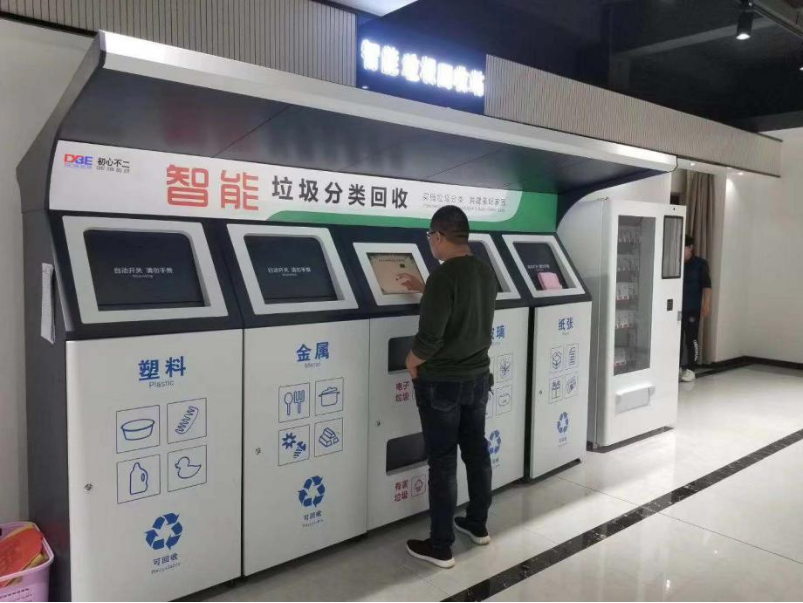
\includegraphics[width=0.95\textwidth,height=0.8\textheight,keepaspectratio]{figures/requirements/image1.png}
    \caption{工作场景：小区垃圾回收系统}
\end{figure}
\subsection{实验目的}
\begin{itemize}
    \item 熟悉 C8051F310 单片机实验平台的 I/O 口、矩阵键盘、数码管、流水灯和蜂鸣器等外设资源的配置方法；
    \item 掌握 4 位数码管动态扫描显示、4$\times$4 矩阵键盘扫描与消抖、74HCT164 串行驱动流水灯等常用接口程序设计方法；
    \item 理解定时器中断和外部中断的工作机制，能够利用 Timer0 构造 1ms 系统节拍，并在主循环状态机中完成倒计时、闪烁和报警等并发任务；
    \item 通过完整汇编程序的编写、构建与调试，提升对模块化程序结构、共享 RAM 状态变量和嵌入式系统故障定位方法的掌握程度。
\end{itemize}

\subsection{实验内容}
本设计基于 C8051F310EVM 实验平台，采用 MCS-51 汇编语言实现小区智能垃圾分类回收系统。系统以四位数码管显示四类垃圾桶剩余容量，以 F1--F4 分类按键完成开盖与投递，以 Timer0 和外部中断分别完成精确定时及提前关盖控制。具体要求如下。

\begin{figure}[H]
    \centering
    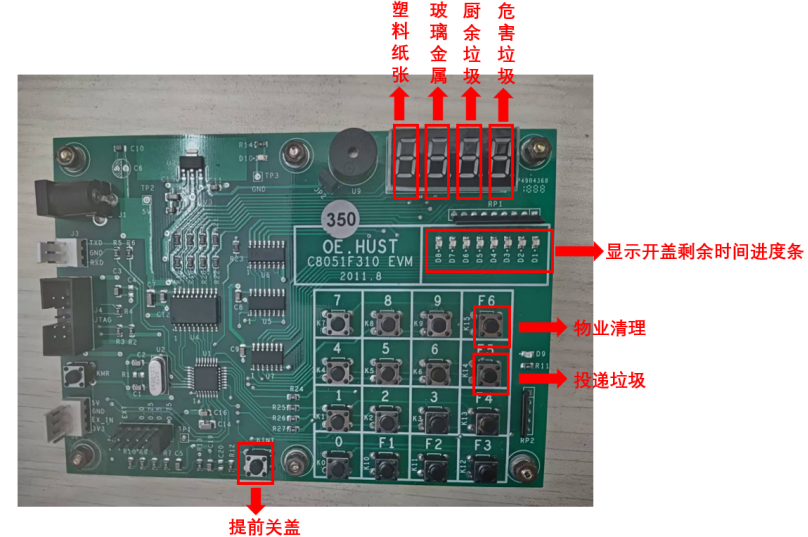
\includegraphics[width=0.95\textwidth,height=0.8\textheight,keepaspectratio]{figures/requirements/image2.png}
    \caption{开发板示意图}
\end{figure}

\subsubsection*{基础部分（满分85）}
\begin{itemize}
    \item 系统将生活垃圾分为“塑料纸张”、“玻璃金属”、“厨余垃圾”和“危害垃圾”四类。上电初始化后，程序随机生成 4 个 $0\sim9$ 的整数，分别作为四个垃圾桶的剩余可投放容量，并在四位数码管上同时显示。
    \item 用户按下 K10--K13（F1--F4）中的某一分类键选择对应垃圾桶。若该桶剩余容量为 0，则认为垃圾桶已满，蜂鸣器鸣响约 1s，对应数码管显示字母 F（FULL），提示结束后恢复原容量显示，桶盖不开启。
    \item 若所选垃圾桶仍有剩余容量，则系统打开对应桶盖，D9 指示灯点亮，开盖时间设定为 8s；开盖期间，对应数码管以 5Hz 频率闪烁，显示该桶当前剩余容量。
    \item 在桶盖打开的 8s 内，用户再次按下同一个分类键表示投入 1 袋垃圾，系统将该桶容量减 1；该操作可重复执行，直至投放完成或容量减至 0。
    \item 桶盖计时由 Timer0 中断完成。程序以 1ms 为系统节拍维护 16 位倒计时变量，要求开盖 8s 后自动关闭桶盖，D9 指示灯熄灭，选中数码管停止闪烁。
\end{itemize}

\subsection{提高部分（申优选做，85分以上）}
在基本功能基础上，当前程序进一步实现了以下扩展功能：
\begin{itemize}
    \item 任一垃圾桶被选择后，四位数码管仍同时刷新显示全部垃圾桶状态；其中被选中的桶位通过 5Hz 闪烁突出显示，未选中的桶位保持正常容量显示。
    \item 桶盖开启期间，流水灯 D1--D8 作为 8s 倒计时进度条显示剩余开盖时间：开盖初始全亮，随后按秒级阈值逐格熄灭，倒计时结束后全部熄灭。
    \item 开盖期间支持 K1--K9 数字键批量投放。按下数字键 $n$ 表示一次投入 $n$ 袋垃圾；若当前容量足够，则容量立即减 $n$；若投入袋数超过剩余容量，则蜂鸣器鸣响约 1s，对应数码管显示 E（ERROR），并关闭桶盖拒绝本次投放。
    \item 若用户在 8s 内已完成投放，可按 Kint 外部中断键提前关盖。外部中断服务程序立即清除开盖状态和倒计时变量，使 D9 与 D1--D8 熄灭，系统返回待机状态。
    \item 增加物业维护功能：按下 K15（F6）后，四个垃圾桶容量统一恢复为 9，同时关闭当前开盖状态并鸣响蜂鸣器作为确认。
    \item 增加计算器个性化功能：按下 K14（F5）进入计算器模式，K0--K9 输入数字，K10--K13 分别表示加、减、乘、除，K15（F6）执行等号运算，K14（F5）用于退格或返回上一步，Kint 用于退出计算器模式并恢复垃圾分类系统。
\end{itemize}

\section{设计思路}
本系统基于 C8051F310 单片机实验平台，采用纯 MCS-51 汇编语言实现。整体程序按照“硬件初始化 + 主循环状态机 + Timer0 周期中断 + INT0 外部中断 + 独立外设驱动模块”的结构组织，将垃圾分类业务、显示刷新、键盘扫描、流水灯输出和计算器扩展功能分离到不同源文件中，便于调试与后续维护。

系统的核心思想是：主循环只负责刷新显示、扫描键盘并根据当前状态执行一次性业务动作；所有需要精确定时的任务交由 Timer0 中断维护；所有需要快速响应的提前关盖动作交由外部中断完成。程序通过片内 RAM 中的状态变量保存四个垃圾桶容量、当前开盖桶号、提示覆盖桶号、错误覆盖桶号、倒计时计数值和计算器模式状态，从而避免长时间阻塞延时，使数码管显示、蜂鸣器报警和按键响应能够同时进行。

整体设计逻辑如下：
\begin{enumerate}
    \item \textbf{系统初始化与随机容量生成模块}：程序复位后首先关闭看门狗，配置 24.5MHz 内部振荡器、端口输出模式、Timer0 工作方式和 INT0 下降沿触发方式。随后初始化片内 RAM 中的容量、键盘、显示、倒计时、报警和计算器状态变量。系统利用 Timer0 自由运行值与端口输入状态组合形成伪随机种子，经乘法、加法和除 10 取余运算后生成 \texttt{CAP0$\sim$CAP3}，作为四个垃圾桶的初始剩余容量。

    \item \textbf{主循环轮询与业务状态机模块}：主循环首先调用流水灯更新函数，再连续刷新四位数码管以保持稳定显示，然后扫描 4$\times$4 矩阵键盘。键盘返回值通过 \texttt{KEYLAST} 进行边沿检测，避免长按造成重复触发。在普通垃圾分类模式下，K10--K13 被解释为四类垃圾桶选择键，K1--K9 被解释为批量投放袋数，K14 进入计算器模式，K15 执行物业清空。主循环根据 \texttt{LIDOPEN}、\texttt{SELBIN} 和容量值判断当前应开盖、投放、拒投还是忽略无效按键。

    \item \textbf{开盖与容量扣减模块}：当用户按下某一分类键且该桶容量不为 0 时，程序设置 \texttt{LIDOPEN=1}，记录当前桶号到 \texttt{SELBIN}，装入 8000ms 倒计时初值，并点亮 D9 表示桶盖打开。开盖期间，再次按下同一分类键将投放 1 袋垃圾；按下 K1--K9 则调用同一容量处理过程一次性投放指定袋数。若当前容量足够，程序直接扣减对应 \texttt{CAP} 变量；若容量不足，则设置 \texttt{ERRBIN} 显示 E，启动 1s 蜂鸣提示，并立即关闭桶盖。

    \item \textbf{Timer0 多任务系统节拍模块}：Timer0 工作在 16 位定时方式，按 1ms 周期重装初值。中断服务程序同时维护三类时间任务：一是递减 \texttt{LIDHI:LIDLO} 组成的 8s 开盖倒计时，计数归零后自动清除开盖状态并熄灭 D9；二是每 100ms 翻转一次 \texttt{BLKFLG}，为选中数码管提供 5Hz 闪烁节拍；三是递减 \texttt{HINTHI:HINTLO} 组成的 1s 提示倒计时，提示结束后关闭蜂鸣器并清除 F/E 覆盖显示。

    \item \textbf{外部中断快速关盖模块}：INT0 与 Kint 按键相连，采用下降沿触发。普通模式下，若桶盖处于打开状态，外部中断服务程序立即清除 \texttt{LIDOPEN}、\texttt{SELBIN} 和倒计时变量，并熄灭 D9，实现不依赖主循环扫描周期的提前关盖。若系统处于计算器模式，Kint 则被复用为退出键，用于清除计算器状态并回到垃圾分类模式。

    \item \textbf{动态数码管显示与覆盖优先级模块}：四位数码管采用分时动态扫描方式显示。普通模式下，各位分别显示 \texttt{CAP0$\sim$CAP3}；显示段码由 \texttt{GET\_SEG} 统一决定。其覆盖优先级为：若当前位等于 \texttt{ERRBIN} 则显示 E，若等于 \texttt{FULLBIN} 则显示 F，若等于开盖桶号且 \texttt{BLKFLG} 处于熄灭相位则显示空白，否则显示正常容量数字。通过这种掩码覆盖方法，程序无需改变容量缓存即可完成错误、满桶和闪烁提示。

    \item \textbf{流水灯倒计时进度条模块}：D1--D8 由 74HCT164 串行移位寄存器驱动，程序使用 \texttt{LEDREG} 保存当前输出掩码，使用 \texttt{LASTBAR} 保存上一次输出值。主循环根据 8000ms 倒计时剩余值映射出 0--8 个亮灯等级，只有掩码变化时才调用移位输出函数，从而减少无效刷新。桶盖关闭时流水灯强制全灭。

    \item \textbf{提示报警与物业清空模块}：当待机状态下选择容量为 0 的垃圾桶时，程序设置 \texttt{FULLBIN} 并启动蜂鸣器，使对应数码管显示 F 约 1s。按下 K15（F6）时，物业清空函数将四个容量变量统一恢复为 9，关闭当前开盖状态，清空流水灯，并鸣响蜂鸣器作为确认反馈。

    \item \textbf{计算器个性化扩展模块}：为体现功能扩展能力，程序加入独立计算器模式。按 K14（F5）进入计算器后，垃圾分类相关状态被暂停并清空提示输出，数码管转为显示计算器缓存 \texttt{CALCD0$\sim$CALCD3}。K0--K9 用于输入最多两位的操作数，K10--K13 分别表示加、减、乘、除，K15 执行等号计算，K14 用于退格或返回。计算完成后，结果通过同一套数码管动态扫描函数显示，Kint 可随时退出并恢复正常垃圾分类模式。
\end{enumerate}

\section{资源分配}
\subsection{I/O口硬件资源分配}
\begin{table}[H]
    \centering
    \small
    \begin{tabular}{|p{2.2cm}|p{1.2cm}|p{7.2cm}|p{2.6cm}|}
        \hline
        I/O引脚 & 方向 & 功能定义 & 有效电平 \\
        \hline
        P0.0 & 输出 & D9 桶盖开启状态指示灯 & 低电平点亮 \\
        \hline
        P0.1 / INT0 & 输入 & Kint 外部中断键，用于提前关盖或退出计算器模式 & 下降沿触发 \\
        \hline
        P0.6, P0.7 & 输出 & 四位数码管位选地址线 BA & 00--11 选择第 0--3 位 \\
        \hline
        P1.0$\sim$P1.7 & 输出 & 数码管段码输出（dp,g,f,e,d,c,b,a 对应位序） & 高电平点亮 \\
        \hline
        P2.0$\sim$P2.3 & 输出 & 4$\times$4 矩阵键盘行扫描线 & 当前扫描行拉低 \\
        \hline
        P2.4$\sim$P2.7 & 输入 & 4$\times$4 矩阵键盘列检测线 & 按下时为低电平 \\
        \hline
        P3.1 & 输出 & 蜂鸣器控制信号 & 高电平鸣响 \\
        \hline
        P3.3 & 输出 & 74HCT164 串行数据输入 DAT，用于 D1--D8 流水灯 & 逐位输出 LED 掩码 \\
        \hline
        P3.4 & 输出 & 74HCT164 移位时钟 CLK，用于 D1--D8 流水灯 & 上升沿移位 \\
        \hline
    \end{tabular}
\end{table}

\subsection{寄存器资源分配}
\begin{table}[H]
    \centering
    \small
    \begin{tabular}{|p{3.8cm}|p{11.2cm}|}
        \hline
        寄存器 & 功能定义 \\
        \hline
        ACC(A) & 主要累加器，用于键值判断、容量计算、段码查表、倒计时比较和中断临时运算 \\
        \hline
        B & 与 ACC 配合完成随机容量生成中的乘除法、计算器运算以及十进制拆分 \\
        \hline
        DPTR & 指向 ROM 查找表，包括数码管段码表、流水灯掩码表和键盘重映射表 \\
        \hline
        R0 & 间接寻址指针或循环计数器，在容量数组访问与 74HCT164 移位输出中使用 \\
        \hline
        R2 & 投放袋数参数，传递给 \texttt{HANDLE\_BAGS} 判断容量是否足够 \\
        \hline
        R3 & 临时保存当前垃圾桶编号，用于容量不足时恢复错误显示桶号 \\
        \hline
        R4, R5, R6 & 数码管消隐延时、计算器结果拆位和短延时循环中的临时寄存器 \\
        \hline
        R7 & 键盘消抖延时循环计数器 \\
        \hline
        PSW & 程序状态字，在中断服务程序中入栈保护，避免影响主程序状态 \\
        \hline
        TH0, TL0 & Timer0 高低字节寄存器，重装 \texttt{0xF806} 形成约 1ms 中断节拍 \\
        \hline
        TMOD, TCON, IE & 定时器工作方式、外部中断触发方式以及中断允许控制寄存器 \\
        \hline
        P0MDOUT--P3MDOUT, P2MDIN, XBR1, OSCICN, PCA0MD & C8051F310 端口模式、交叉开关、内部振荡器和看门狗相关配置寄存器 \\
        \hline
    \end{tabular}
\end{table}

\subsection{片内RAM资源分配}
\begin{table}[H]
    \centering
    \small
    \begin{tabular}{|p{3.2cm}|p{11.8cm}|}
        \hline
        存储单元 & 功能定义 \\
        \hline
        30H$\sim$33H & \texttt{CAP0$\sim$CAP3}，四个分类垃圾桶的剩余容量，取值范围为 $0\sim9$ \\
        \hline
        34H, 35H & \texttt{KEYNOW}, \texttt{KEYLAST}，保存当前键号和上一轮键号，用于按键边沿检测 \\
        \hline
        36H & \texttt{ROWIDX}，矩阵键盘扫描当前行号 \\
        \hline
        37H, 38H & \texttt{TMP}, \texttt{CNT}，通用临时变量和主循环刷新计数器 \\
        \hline
        39H, 3BH & \texttt{LEDREG}, \texttt{LASTBAR}，当前流水灯输出掩码和上一次输出掩码 \\
        \hline
        42H, 43H & \texttt{LIDLO}, \texttt{LIDHI}，16 位开盖倒计时，单位为 ms，初值为 8000ms \\
        \hline
        44H, 45H & \texttt{BLKDIV}, \texttt{BLKFLG}，100ms 分频计数与 5Hz 闪烁相位标志 \\
        \hline
        46H, 47H & \texttt{HINTLO}, \texttt{HINTHI}，16 位蜂鸣器和 F/E 提示倒计时，单位为 ms，初值为 1000ms \\
        \hline
        4DH & \texttt{LIDOPEN}，桶盖开启状态标志，0 表示关闭，1 表示打开 \\
        \hline
        4EH & \texttt{SELBIN}，当前被选中的垃圾桶编号，\texttt{0xFF} 表示无选中桶 \\
        \hline
        4FH & \texttt{FULLBIN}，当前显示 F（FULL）的桶号，\texttt{0xFF} 表示无覆盖显示 \\
        \hline
        50H & \texttt{ERRBIN}，当前显示 E（ERROR）的桶号，\texttt{0xFF} 表示无覆盖显示 \\
        \hline
        51H--53H & \texttt{CALCMODE}, \texttt{CALCSTATE}, \texttt{CALCOP}，计算器模式、输入阶段和运算符状态 \\
        \hline
        54H--57H & \texttt{OP1}, \texttt{OP2}, \texttt{DIGCNT}, \texttt{CALCNEG}，计算器两个操作数、当前输入位数和负号标志 \\
        \hline
        58H, 59H & \texttt{RESLO}, \texttt{RESHI}，计算器 16 位结果缓存 \\
        \hline
        5AH--5DH & \texttt{CALCD0$\sim$CALCD3}，计算器模式下的四位数码管显示缓存，支持数字、空白、负号和 E \\
        \hline
    \end{tabular}
\end{table}

\newpage
\section{流程图}
\noindent 系统运行流程可分为三个相互配合的部分：主程序负责垃圾分类业务状态判断和按键分发，Timer0 与 INT0 负责倒计时、闪烁、报警和提前关盖等实时任务，显示驱动负责四位数码管覆盖显示及 D1--D8 流水灯进度刷新。以下流程图分别给出这三部分的具体执行过程。

\subsection{主程序状态轮询架构流程图}
\begin{figure}[H]
    \centering
    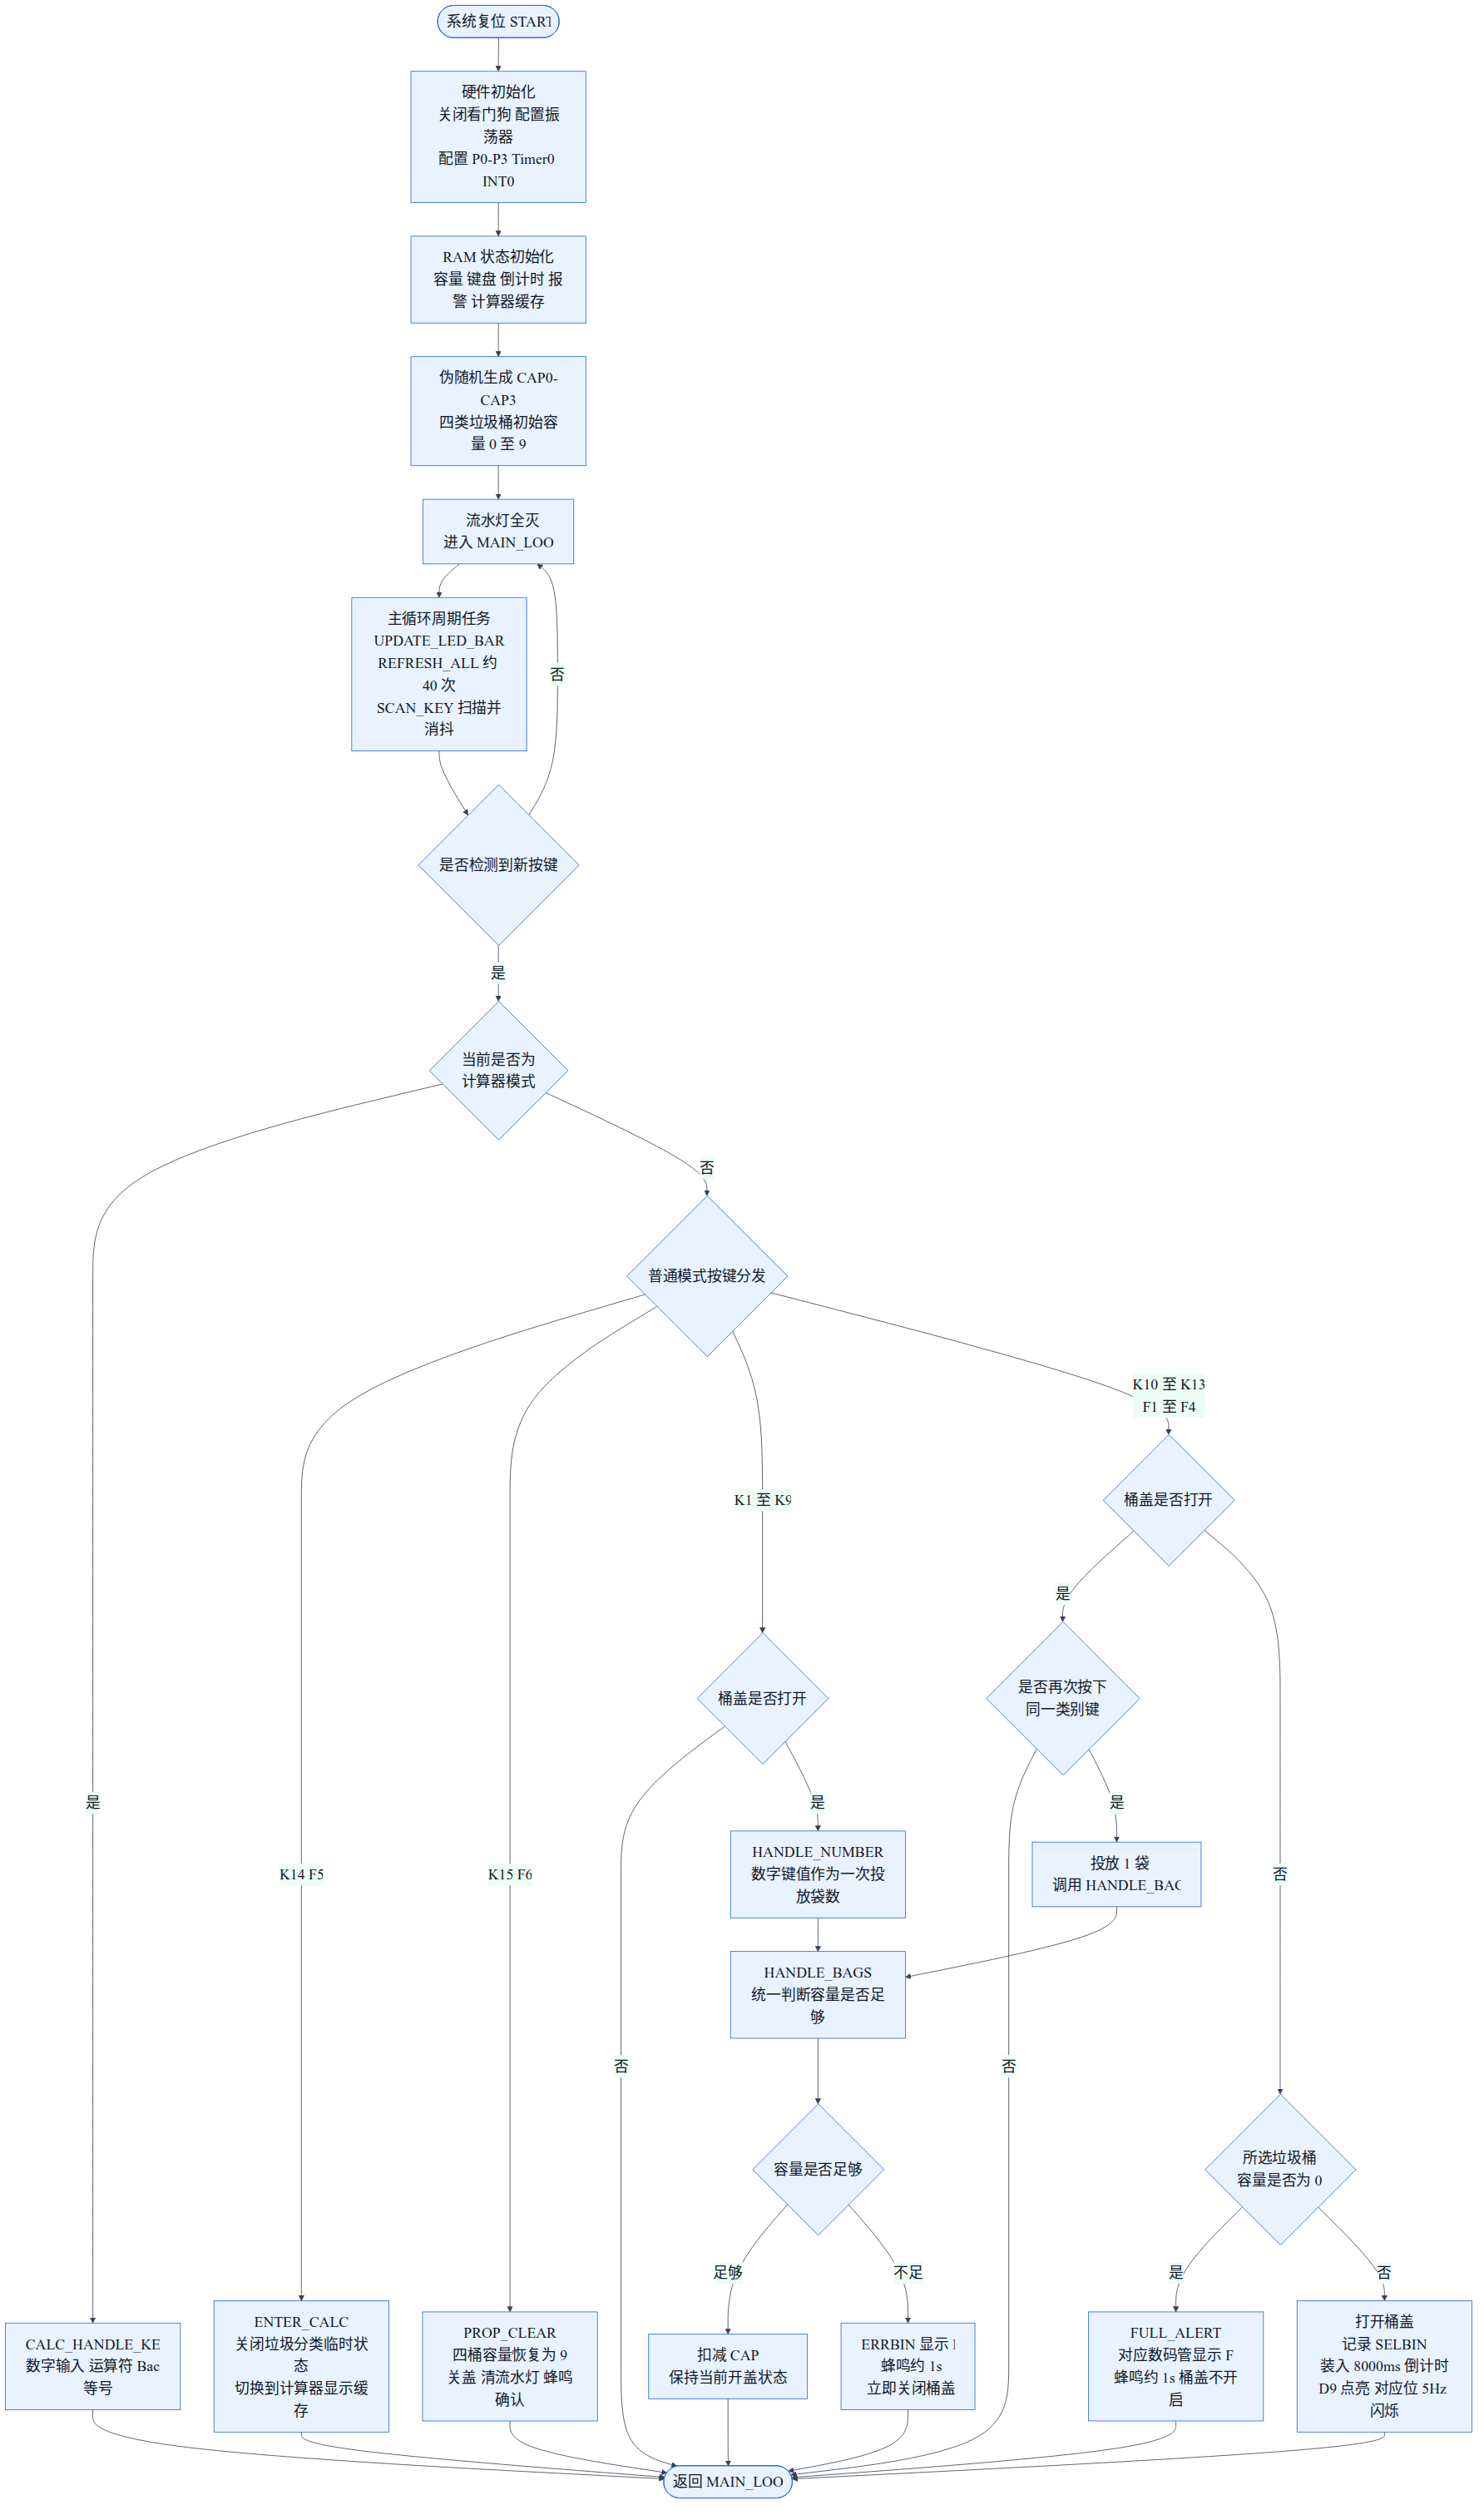
\includegraphics[width=\textwidth,height=0.82\textheight,keepaspectratio]{figures/flowchart/main_state.png}
    \caption{主程序状态轮询与垃圾分类业务判别流程图}
\end{figure}

\newpage
\subsection{定时器/外部中断并行处理流程图}
\begin{figure}[H]
    \centering
    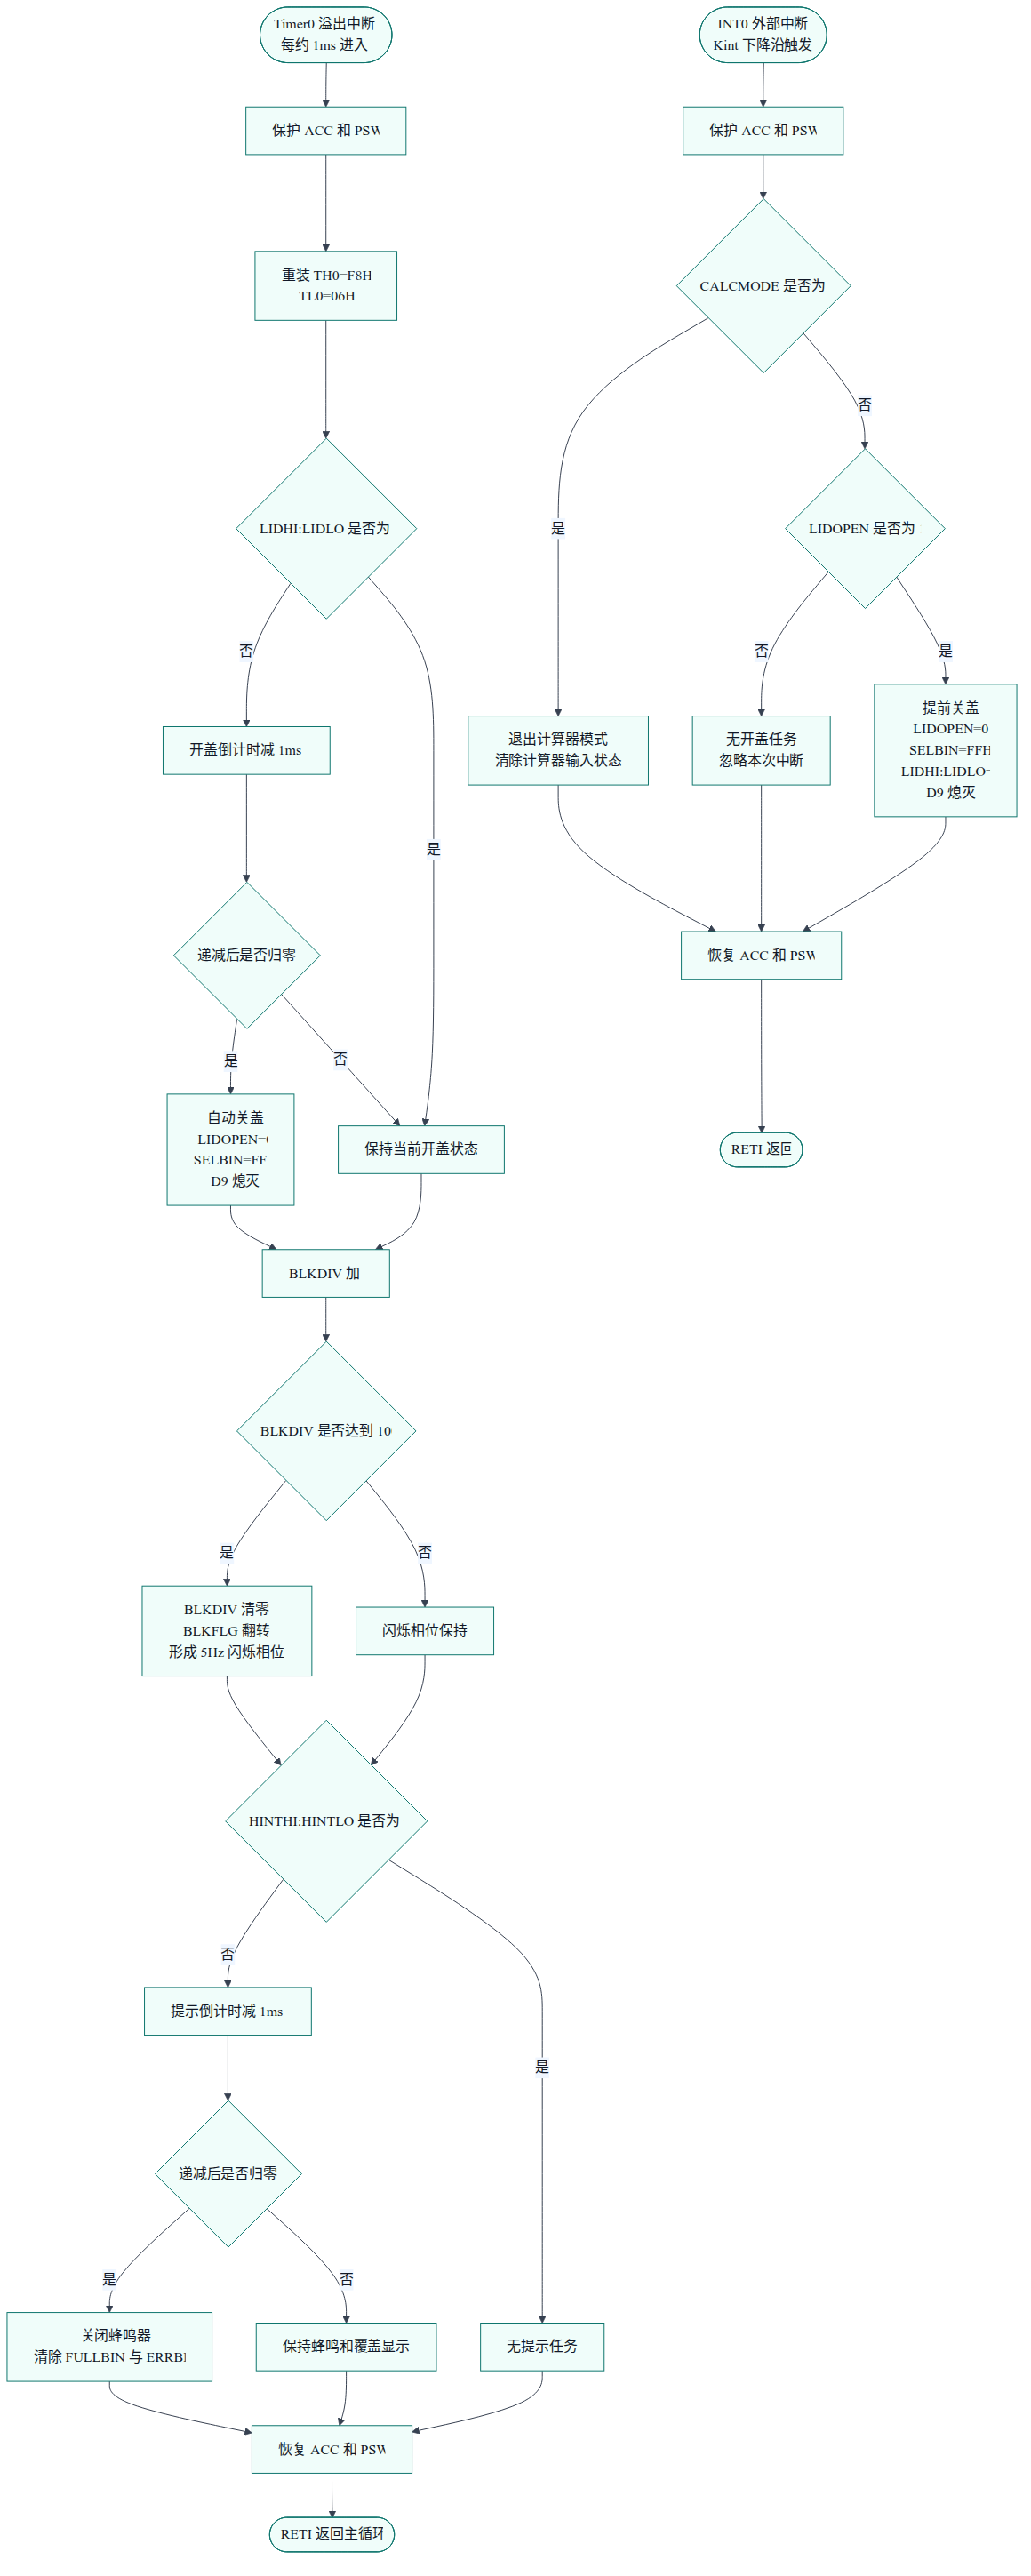
\includegraphics[width=\textwidth,height=0.82\textheight,keepaspectratio]{figures/flowchart/interrupt_timing.png}
    \caption{Timer0 系统节拍与 INT0 外部中断并行处理流程图}
\end{figure}

\newpage
\subsection{动态显示与流水灯刷新流程图}
\begin{figure}[H]
    \centering
    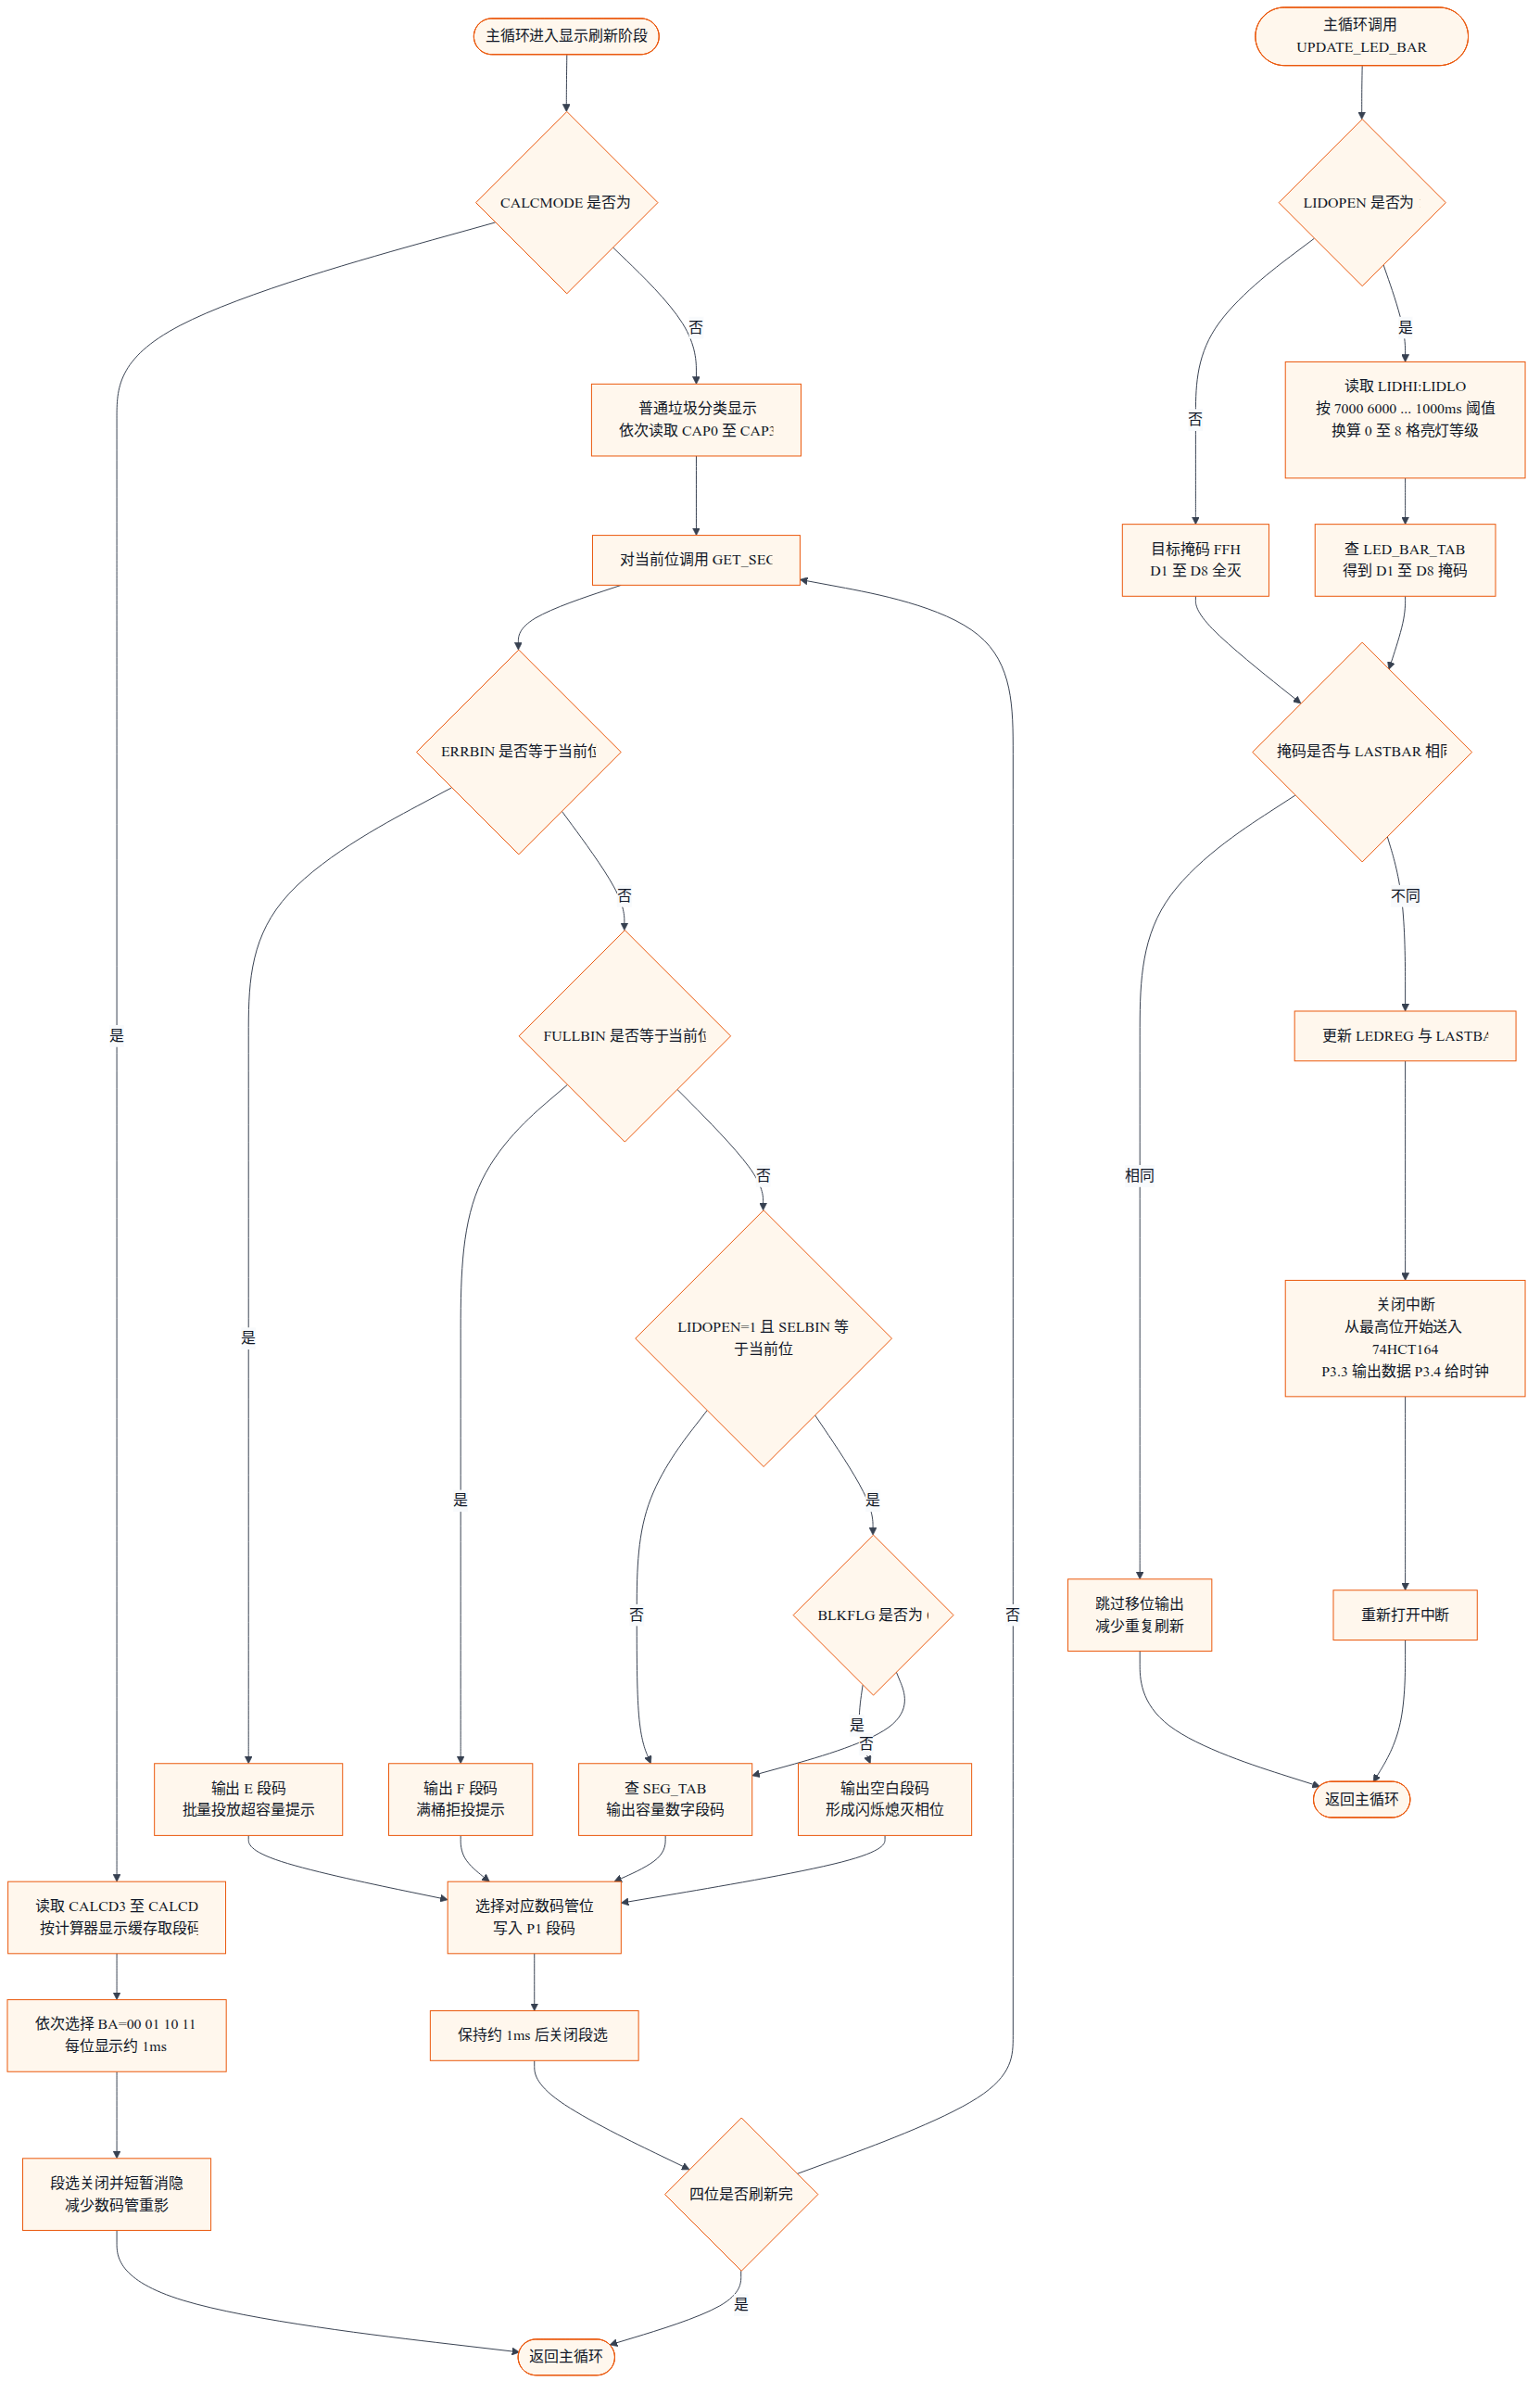
\includegraphics[width=\textwidth,height=0.82\textheight,keepaspectratio]{figures/flowchart/display_led.png}
    \caption{数码管覆盖显示与 D1--D8 流水灯进度条刷新流程图}
\end{figure}
\clearpage

\section{源代码 （含文件头说明、语句行注释）}
本系统源码采用多文件汇编结构组织。公共头文件定义特殊功能寄存器和片内 RAM 变量，启动文件完成硬件初始化，中断、显示、键盘、流水灯、查表、主状态机和计算器扩展分别放在独立模块中。各源文件开头均说明了模块用途、硬件连接或导出函数，关键语句处也保留了必要注释，便于结合前文设计思路阅读。

\subsection{源码文件组织}
\begin{table}[H]
    \centering
    \small
    \begin{tabular}{|p{4.2cm}|p{10.8cm}|}
        \hline
        文件 & 主要功能 \\
        \hline
        \texttt{inc/sfr.inc} & C8051F310 标准及扩展特殊功能寄存器、位地址和硬件别名定义。 \\
        \hline
        \texttt{inc/iram.inc} & 片内 RAM 共享变量地址定义，包括容量、键盘、倒计时、提示和计算器缓存。 \\
        \hline
        \texttt{src/vectors.asm} & 复位向量、INT0 外部中断向量和 Timer0 中断向量。 \\
        \hline
        \texttt{src/init.asm} & 单片机初始化、端口模式配置、Timer0/INT0 配置、随机容量生成和程序入口。 \\
        \hline
        \texttt{src/isr.asm} & Kint 提前关盖外部中断服务程序与 1ms Timer0 系统节拍中断服务程序。 \\
        \hline
        \texttt{src/display.asm} & 四位数码管动态扫描、F/E 覆盖显示、5Hz 闪烁显示和计算器显示缓存转换。 \\
        \hline
        \texttt{src/keypad.asm} & 4$\times$4 矩阵键盘扫描、消抖和物理键位到逻辑键号的映射。 \\
        \hline
        \texttt{src/led\_bar.asm} & D1--D8 流水灯进度条计算和 74HCT164 串行移位输出。 \\
        \hline
        \texttt{src/tables.asm} & 数码管段码表、流水灯等级掩码表和键盘重映射表。 \\
        \hline
        \texttt{src/main.asm} & 主循环、垃圾桶开盖状态机、容量扣减、满桶/错误提示和物业清空。 \\
        \hline
        \texttt{src/calculator.asm} & F5 进入的计算器扩展模式，包括输入、退格、四则运算和结果显示。 \\
        \hline
    \end{tabular}
\end{table}

\lstset{
    language={[x86masm]Assembler},
    basicstyle=\scriptsize\ttfamily,
    numbers=left,
    numberstyle=\tiny,
    stepnumber=1,
    numbersep=6pt,
    frame=single,
    breaklines=true,
    columns=flexible,
    keepspaces=true,
    showstringspaces=false,
    commentstyle=\upshape,
    tabsize=4
}

\subsection{公共头文件}
\lstinputlisting[caption={特殊功能寄存器定义：inc/sfr.inc}]{codes/Core/inc/sfr.inc}
\lstinputlisting[caption={片内 RAM 共享变量定义：inc/iram.inc}]{codes/Core/inc/iram.inc}

\subsection{启动与中断向量}
\lstinputlisting[caption={中断向量表：src/vectors.asm}]{codes/Core/src/vectors.asm}
\lstinputlisting[caption={硬件初始化与程序入口：src/init.asm}]{codes/Core/src/init.asm}

\subsection{中断服务程序}
\lstinputlisting[caption={外部中断与 Timer0 中断：src/isr.asm}]{codes/Core/src/isr.asm}

\subsection{外设驱动模块}
\lstinputlisting[caption={四位数码管动态显示驱动：src/display.asm}]{codes/Core/src/display.asm}
\lstinputlisting[caption={矩阵键盘扫描驱动：src/keypad.asm}]{codes/Core/src/keypad.asm}
\lstinputlisting[caption={D1--D8 流水灯驱动：src/led\_bar.asm}]{codes/Core/src/led_bar.asm}
\lstinputlisting[caption={ROM 查找表：src/tables.asm}]{codes/Core/src/tables.asm}

\subsection{业务状态机与扩展功能}
\lstinputlisting[caption={垃圾分类主状态机：src/main.asm}]{codes/Core/src/main.asm}
\lstinputlisting[caption={计算器扩展状态机：src/calculator.asm}]{codes/Core/src/calculator.asm}

\section{程序测试方法与结果}
本节对程序的构建结果和板级功能进行测试。测试平台为 C8051F310EVM，观察对象包括四位数码管、D1--D8 流水灯、D9 桶盖状态灯和蜂鸣器，测试内容覆盖基础要求、提高要求和个性化扩展功能。

\subsection{编译测试}
本工程采用 \texttt{sdas8051} 汇编器和 \texttt{sdld} 链接器构建，执行工程构建脚本后，9 个汇编源文件均成功生成目标文件，并链接得到 \texttt{c8051f310.hex}。当前构建输出无 Error，未出现 Warning 提示，生成的 Intel HEX 文件大小约为 5.0KB。

根据链接生成的 \texttt{c8051f310.map} 文件统计，程序各代码段和查表数据段实际占用约 2111 字节，最高使用代码地址约为 \texttt{0x0B7A}，低于 C8051F310 本实验可用的 8KB 程序空间限制，容量满足下载和运行要求。

\subsection{功能测试项目}
\begin{table}[H]
    \centering
    \small
    \begin{tabular}{|p{2.5cm}|p{4.3cm}|p{6.5cm}|}
        \hline
        测试项目 & 操作方法 & 预期现象 \\
        \hline
        上电初始化 & 烧录程序后复位实验板 & 四位数码管显示 4 个 $0\sim9$ 的容量值，蜂鸣器关闭，D9 熄灭，D1--D8 流水灯熄灭。 \\
        \hline
        F1--F4 开盖 & 按下 K10--K13（F1--F4）中的任一分类键 & 若对应容量大于 0，则 D9 点亮，桶盖进入 8s 开启状态，选中数码管以约 5Hz 闪烁，流水灯开始显示倒计时进度。 \\
        \hline
        单袋投递 & 开盖后再次按下同一分类键 & 当前垃圾桶容量减少 1，其它垃圾桶容量保持不变。 \\
        \hline
        数字键多袋投递 & 开盖后按 K1--K9 & 当前垃圾桶容量按数字键值一次性减少对应袋数。 \\
        \hline
        超量投递 & 开盖后按下大于剩余容量的数字键 & 容量不变，对应数码管显示 E，蜂鸣器鸣响约 1s，并立即关闭桶盖。 \\
        \hline
        满桶拒绝 & 将某桶容量投至 0 后，再按对应 F 键 & 系统不开盖，对应数码管显示 F，蜂鸣器鸣响约 1s 后恢复显示 0。 \\
        \hline
        自动关盖 & 开盖后不再操作 & 约 8s 后自动关盖，D9 熄灭，D1--D8 进度条结束，数码管停止闪烁。 \\
        \hline
        提前关盖 & 开盖期间按 Kint & 外部中断立即清除开盖倒计时，D9 熄灭，流水灯全灭，系统返回待机状态。 \\
        \hline
        物业清空 & 按 K15（F6） & 四个垃圾桶容量恢复为 9，当前开盖状态被清除，蜂鸣器短响确认。 \\
        \hline
        计算器模式 & 按 K14（F5）进入，使用 K0--K9 和 K10--K15 操作 & 数码管切换为计算器显示，支持数字输入、四则运算、退格和等号；按 Kint 后退出并恢复垃圾分类显示。 \\
        \hline
    \end{tabular}
\end{table}

\subsection{测试结果}
按照表中项目逐项测试后，系统表现与预期一致。上电或复位后，四个垃圾桶容量能够正常初始化并显示；按下 F1--F4 分类键后，容量非零的垃圾桶能够正常开盖，D9、流水灯和选中数码管闪烁状态均能正确联动。开盖期间，同类键单袋投递和 K1--K9 数字键多袋投递均能正确扣减容量。

异常场景测试中，满桶状态下系统能够拒绝开盖并显示 F；批量投放超过剩余容量时，系统能够显示 E、蜂鸣提示并立即关闭桶盖，且容量保持不变。定时测试中，8s 自动关盖准确发生；外部中断测试中，Kint 能够立即提前关盖，说明 Timer0 中断和 INT0 中断能够与主循环状态机正确配合。

扩展功能测试中，K15（F6）物业清空能够将四个容量统一恢复为 9；K14（F5）计算器模式能够正常进入和退出，并完成基本四则运算。综合测试表明，当前程序已实现实验任务要求的基础功能和提高功能，运行过程中未发现明显显示冲突、误触发或状态无法恢复的问题。




\section{实验问题分析与对策}

\begin{enumerate}
    \item \textbf{矩阵键盘物理扫描顺序与实验按键编号不一致}：
    \begin{itemize}
        \item \textbf{原因分析}：4$\times$4 矩阵键盘按行列扫描时，程序首先得到的是“行号乘以 4 再加列号”的自然扫描码。该顺序与实验资料中标注的 K0--K15 逻辑编号并不完全一致，如果直接使用扫描码，会导致 K10--K13、K14、K15 等功能键与实际按键含义错位，从而影响垃圾桶分类选择、计算器入口和物业清空功能。
        \item \textbf{解决方法}：在键盘扫描模块中增加 \texttt{KEY\_REMAP\_TAB} 查表映射。程序完成行列扫描和消抖后，先计算自然扫描码，再通过该表转换为实验 PDF 中的逻辑键号，使 K10--K13 正确对应 F1--F4，K14 对应 F5，K15 对应 F6。主循环只处理重映射后的键号，从而避免业务逻辑与物理键盘布局耦合。
    \end{itemize}

    \item \textbf{机械按键抖动与长按重复触发}：
    \begin{itemize}
        \item \textbf{原因分析}：矩阵键盘为机械按键，按下和释放瞬间会出现电平抖动；同时主循环会周期性扫描键盘，如果不区分“刚按下”和“持续按住”，长按某个分类键或数字键可能被识别为多次输入，造成容量连续扣减或功能重复触发。
        \item \textbf{解决方法}：在 \texttt{SCAN\_KEY} 中加入约 30ms 的消抖等待，并在主循环中使用 \texttt{KEYNOW} 与 \texttt{KEYLAST} 做边沿检测。只有当前键号与上一轮不同，且不是无键状态时，才认为产生一次新按键事件；当扫描结果为无键时，再将 \texttt{KEYLAST} 恢复为 \texttt{0xFF}。这样既能过滤抖动，也能避免长按期间反复触发。
    \end{itemize}

    \item \textbf{中断与主循环共享 16 位状态变量}：
    \begin{itemize}
        \item \textbf{原因分析}：Timer0 中断每 1ms 修改开盖倒计时 \texttt{LIDHI:LIDLO}、提示倒计时 \texttt{HINTHI:HINTLO} 和闪烁标志；主循环在开盖、满桶报警、超量投放和物业清空时也会写这些变量。由于 8051 写 16 位变量需要分两次写高低字节，若写入过程中被 Timer0 中断打断，可能造成倒计时高低字节短暂不一致。
        \item \textbf{解决方法}：在主循环需要重新装载或清零 16 位倒计时变量时，先短暂关闭总中断 \texttt{EA}，完成低字节和高字节写入后再打开 \texttt{EA}。中断服务程序内部只按固定顺序递减变量，主循环与中断之间通过这种短临界区方式避免读写冲突。
    \end{itemize}

    \item \textbf{容量不足时的状态恢复问题}：
    \begin{itemize}
        \item \textbf{原因分析}：数字键批量投放时，如果输入袋数超过当前垃圾桶剩余容量，仅显示 E 而继续保持开盖状态，会让用户误以为仍可继续投放，与“拒绝本次投放”的业务含义不一致，也容易造成后续按键状态混乱。
        \item \textbf{解决方法}：在 \texttt{HANDLE\_BAGS} 中检测到容量不足后，程序设置 \texttt{ERRBIN} 显示 E，启动 1s 蜂鸣提示，并立即清除 \texttt{LIDOPEN}、\texttt{SELBIN} 和 \texttt{LIDHI:LIDLO}，同时熄灭 D9。这样系统在错误提示结束后自然回到关盖待机状态，容量值保持不变。
    \end{itemize}

    \item \textbf{动态数码管刷新时出现重影风险}：
    \begin{itemize}
        \item \textbf{原因分析}：四位数码管采用分时动态扫描，如果在切换位选时 P1 段码仍保持上一位的输出，可能在极短时间内把上一位段码显示到下一位，表现为轻微重影。开盖闪烁、F/E 覆盖显示和计算器显示复用同一套数码管驱动时，这一问题更明显。
        \item \textbf{解决方法}：在 \texttt{REFRESH\_ALL} 中切换每一位前先将 \texttt{P1} 清零关闭段选，并调用短消隐延时 \texttt{DISPLAY\_BLANK\_GAP}，待位选地址稳定后再输出新的段码。显示覆盖优先级统一放在 \texttt{GET\_SEG} 中处理，保证 E、F、闪烁空白和正常数字不会互相覆盖。
    \end{itemize}

    \item \textbf{流水灯串行移位输出可能被中断打断}：
    \begin{itemize}
        \item \textbf{原因分析}：D1--D8 流水灯由 74HCT164 串行移位寄存器驱动，程序需要连续输出 8 位数据和时钟脉冲。如果移位过程中发生 Timer0 中断，P3.3/P3.4 的数据和时钟时序可能被拉长，造成流水灯状态短暂异常。
        \item \textbf{解决方法}：在 \texttt{SHIFT\_LED\_BAR} 中移位输出前关闭总中断 \texttt{EA}，连续完成 8 位数据发送后再打开中断。由于该过程很短，不会明显影响 1ms 系统节拍，却能保证 74HCT164 获得完整稳定的移位时序。
    \end{itemize}

\end{enumerate}

\vspace{2cm}
\noindent
本人承诺:本报告内容真实，无伪造数据，无抄袭他人成果。本人完全了解学校相关规定，如若违反，愿意承担其后果。

\vspace{1cm}
\noindent
签字：\hspace{3cm} 陈恪瑾 \hspace{3cm} 2026年4月26日

\end{document}
